% polynome1
%-------------------
\documentclass[tikz]{standalone}
\usepackage{amsmath}
\usepackage{times}
\usepackage{txfonts}
\usepackage{pgfplots}
\usepackage{csvsimple}
\usetikzlibrary{arrows,intersections,math}
\newcommand{\teiler}{40}
\begin{document}
	%Übertragen von den Zahlen 
	%\textcolor{blue}{2}, \textcolor{blue}{1}, \textcolor{blue}{5} 
	%als $ p(x) = \textcolor{blue}{2}x^2 + \textcolor{blue}{1}x + \textcolor{blue}{5} $.\newline
	%Versende $ (p(1),p(2),...,p(7)) = (\textcolor{green}{8}, 
	%	\textcolor{green}{15}, \textcolor{green}{26},
	%	\textcolor{green}{ 41}, \textcolor{green}{60}, 
	%	\textcolor{green}{83}, \textcolor{green}{110})$


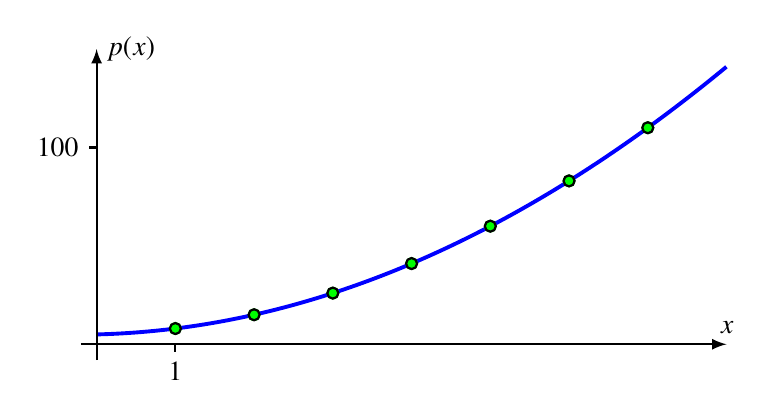
\begin{tikzpicture}[>=latex,thick]

\draw[color=blue, line width=1.4pt] 
plot[domain=0:8, samples=100]
	({\x},{(2*\x^2+1*\x+5)/\teiler});
\draw[->] (-0.2,0) -- (8,0) coordinate[label={$x$}];
\draw[->] (0,-0.2) -- (0,150/\teiler) coordinate[label={right:$p(x)$}];
\def\punkt#1{
	\fill[color=green] #1 circle[radius=0.08];
	\draw #1 circle[radius=0.07];
}
\punkt{(1,8/\teiler)}
\punkt{(2,15/\teiler)}
\punkt{(3,26/\teiler)}
\punkt{(4,41/\teiler)}
\punkt{(5,60/\teiler)}
\punkt{(6,83/\teiler)}
\punkt{(7,110/\teiler)}
%\draw[color=gray,line width=1pt,dashed] 
%plot[domain=0.5:7, samples=100]
%({\x},{(0.1958*\x^2-1.2875*\x+3.0417)});
%\def\erpunkt#1{
%	\fill[color=red] #1 circle[radius=0.08];
%	\draw #1 circle[radius=0.07];
%}
%\erpunkt{(2,50/\teiler)}
%\erpunkt{(3,0.9414)}
%\punkt{(4,41/\teiler)}
%\punkt{(5,60/\teiler)}

\draw(0,100/\teiler) -- (-0.1,100/\teiler) coordinate[label={left:$100$}];
\draw(1,0) -- (1,-0.1) coordinate[label={below:$1$}];




\end{tikzpicture}
\end{document}

